\subsection{Part 2: Stopping voltage and photocurrent as a function of intensity.}

Table \ref{tab:results2} lists the stopping voltages and photocurrents for different intensity settings.



\begin{table}

    \caption{Stopping Voltage and Photocurrent as a function of intensity.}
    \label{tab:results2}
    \centering
    \begin{tabular}{|c|c|c|}
        \hline
        \rowcolor{lightgray} Intensity & Stopping Voltage         & Current (Voltage across 100 k$\Omega$ resistor) \\
        \hline
        \rowcolor{red!80} 3            & 0.947739 $\pm$ 0.0000005 & 0.218967 $\pm$ 0.0000005                        \\
        \rowcolor{red!60} 2            & 0.948277 $\pm$ 0.0000005 & 0.188794 $\pm$ 0.0000005                        \\
        \rowcolor{red!40} 1            & 0.943390 $\pm$ 0.0000005 & 0.173533 $\pm$ 0.0000005                        \\
        \rowcolor{red!20} 0            & 0.943300 $\pm$ 0.0000005 & 0.160800 $\pm$ 0.0000005                        \\
        \hline
    \end{tabular}
\end{table}

These values are graphed in Figure \ref{fig:voltage_vs_intensity}. Notice that the uncertainties, although present in the table, are too small to be seen in the graph.

The general trend that can be observed is that the stopping voltage stays relatively constant, while the photocurrent increases with intensity.

\begin{figure}[H]
    \centering
    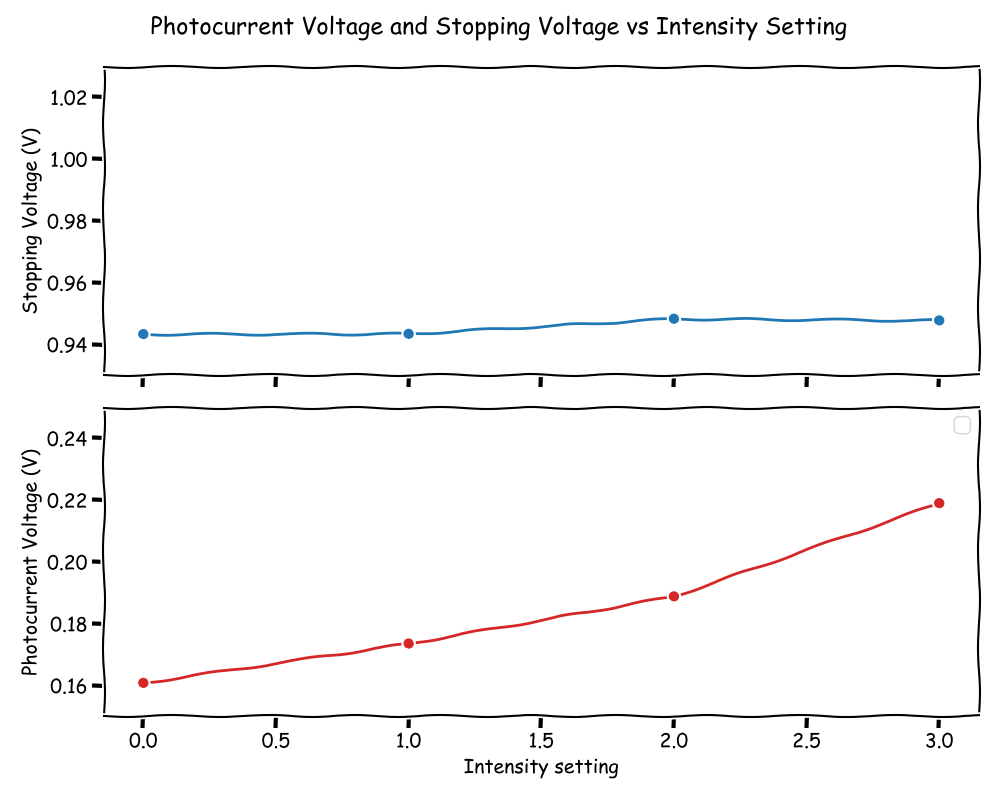
\includegraphics[width=0.8\textwidth]{Results/Part2/Part2.png}
    \caption{Stopping Voltage vs. Intensity}
    \label{fig:voltage_vs_intensity}
\end{figure}


\subsubsection{Relation to the original theory}

The trend in the increasing photocurrent with intensity is consistent with the theory.
The theory says that electrons are freed after they have absorbed enough energy to overcome the work function of the metal.
If a highier intensity is applied, corresponding to a higher number of photons, more electrons will be freed, and thus the photocurrent will increase.

However, this theory postulates that the energy is absorbed continuously from the light, which does not explain why the stopping voltage remains constant.

\subsubsection{Einstein's explanation}

Einstein's explanation of the photoelectric effect is that light is quantized into photons, which have a discrete energy.
The energy of a photon is given by $E = hf$, where $h$ is Planck's constant and $f$ is the frequency of the light.

This gives the insight that the energy carried by the photon and absorbed by the electron is proportional to the frequency (and wavelength) of the light, and not the intensity.
Thus, the stopping voltage is constant, as it is determined by the energy of the photons, and not the number of photons that arrive at the metallic surface.

The same argument about the relationship between increasing intensity and greater photocurrent can be made, as the number of photons arriving at the surface is proportional to the intensity.

Thus, we can conclude that Einstein's explanation is more consistent with the data than the original theory.

